\documentclass[12pt, titlepage]{article}

\usepackage{fullpage}
\usepackage[round]{natbib}
\usepackage{multirow}
\usepackage{booktabs}
\usepackage{tabularx}
\usepackage{longtable}
\usepackage{graphicx}
\usepackage{float}
\usepackage{hyperref}
\hypersetup{
    colorlinks,
    citecolor=blue,
    filecolor=black,
    linkcolor=red,
    urlcolor=blue
}
\setlength{\parindent}{0pt}
\setlength{\parskip}{0.75em}

\input{../../Comments.text}
\input{../../Common.text}

\newcounter{acnum}
\newcommand{\actheacnum}{AC\theacnum}
\newcommand{\acref}[1]{AC\ref{#1}}

\newcounter{ucnum}
\newcommand{\uctheucnum}{UC\theucnum}
\newcommand{\uref}[1]{UC\ref{#1}}

\newcounter{mnum}
\newcommand{\mthemnum}{M\themnum}
\newcommand{\mref}[1]{\hyperref[#1]{M\ref*{#1}}}
\setlength{\parindent}{0pt}
\setlength{\parskip}{0.75em}
\begin{document}

\title{Module Guide for \progname{}} 
\author{\authname}
\date{\today}

\maketitle

\pagenumbering{roman}

\section{Revision History}

\begin{tabularx}{\textwidth}{p{3cm}p{2cm}X}
\toprule {\bf Date} & {\bf Version} & {\bf Notes}\\
\midrule
Date 1 & 1.0 & Notes\\
Date 2 & 1.1 & Notes\\
\bottomrule
\end{tabularx}

\newpage

\section{Reference Material}

This section records information for easy reference. 

\subsection{Abbreviations and Acronyms}

\renewcommand{\arraystretch}{1.2}
\begin{tabular}{l l} 
  \toprule		
  \textbf{symbol} & \textbf{description}\\
  \midrule 
  AC & Anticipated Change\\
  DAG & Directed Acyclic Graph \\
  M & Module \\
  MG & Module Guide \\
  OS & Operating System \\
  R & Requirement\\
  SC & Scientific Computing \\
  SRS & Software Requirements Specification\\
  \progname & Explanation of program name\\
  UC & Unlikely Change \\
  \wss{etc.} & \wss{...}\\
  \bottomrule
\end{tabular}\\

\newpage

\tableofcontents

\listoftables

\listoffigures

\newpage

\pagenumbering{arabic}

\section{Introduction}

Decomposing a system into modules is a commonly accepted approach to developing
software.  A module is a work assignment for a programmer or programming
team~\citep{ParnasEtAl1984}.  We advocate a decomposition
based on the principle of information hiding~\citep{Parnas1972a}.  This
principle supports design for change, because the ``secrets'' that each module
hides represent likely future changes.  Design for change is valuable in SC,
where modifications are frequent, especially during initial development as the
solution space is explored.  

Our design follows the rules layed out by \citet{ParnasEtAl1984}, as follows:
\begin{itemize}
\item System details that are likely to change independently should be the
  secrets of separate modules.
\item Each data structure is implemented in only one module.
\item Any other program that requires information stored in a module's data
  structures must obtain it by calling access programs belonging to that module.
\end{itemize}

After completing the first stage of the design, the Software Requirements
Specification (SRS), the Module Guide (MG) is developed~\citep{ParnasEtAl1984}. The MG
specifies the modular structure of the system and is intended to allow both
designers and maintainers to easily identify the parts of the software.  The
potential readers of this document are as follows:

\begin{itemize}
\item New project members: This document can be a guide for a new project member
  to easily understand the overall structure and quickly find the
  relevant modules they are searching for.
\item Maintainers: The hierarchical structure of the module guide improves the
  maintainers' understanding when they need to make changes to the system. It is
  important for a maintainer to update the relevant sections of the document
  after changes have been made.
\item Designers: Once the module guide has been written, it can be used to
  check for consistency, feasibility, and flexibility. Designers can verify the
  system in various ways, such as consistency among modules, feasibility of the
  decomposition, and flexibility of the design.
\end{itemize}

The rest of the document is organized as follows. Section
\ref{SecChange} lists the anticipated and unlikely changes of the software
requirements. Section \ref{SecMH} summarizes the module decomposition that
was constructed according to the likely changes. Section \ref{SecConnection}
specifies the connections between the software requirements and the
modules. Section \ref{SecMD} gives a detailed description of the
modules. Section \ref{SecTM} includes two traceability matrices. One checks
the completeness of the design against the requirements provided in the SRS. The
other shows the relation between anticipated changes and the modules. Section
\ref{SecUse} describes the use relation between modules.



\section{Anticipated and Unlikely Changes} \label{SecChange}
This section identifies potential changes to the FPVR system that may affect its software architecture. 
These changes are classified into anticipated changes, which the modular design should accommodate, and 
unlikely changes, which are expected to remain stable throughout development.

The classification is based on the requirements and constraints established in the FPVR Software 
Requirements Specification (SRS). Anticipated changes guide the separation of responsibilities between 
modules, while unlikely changes establish architectural decisions that do not require the same degree of 
flexibility.

\subsection{Anticipated Changes} \label{SecAchange}

Anticipated changes represent aspects of the system's requirements, design, or
 implementation that may evolve as development progresses. Following the principle 
 of information hiding, these decisions should be encapsulated within individual 
 modules wherever possible, minimizing the impact of modifications on the rest of the system.

\begin{description}

\item[\refstepcounter{acnum} \actheacnum \label{acController}:]
The controller input mappings, calibration procedures, and integration
methods may change as different supported controllers are tested.
(Related SRS: FR-UI-02--04, NFR-COMP-01.)

\item[\refstepcounter{acnum} \actheacnum \label{acPhysics}:]
The algorithms and parameters used to simulate drone thrust, gravity,
rotation, and momentum may change to improve flight realism and
responsiveness. (Related SRS: FR-FLT-01--06.)

\item[\refstepcounter{acnum} \actheacnum \label{acEnvironment}:]
Training environment layouts, obstacles, and checkpoint configurations
may change as new courses are developed and user feedback is collected.
(Related SRS: FR-LVL-01--07, FR-CHK-01.)

\item[\refstepcounter{acnum} \actheacnum \label{acCheckpoint}:]
The internal data structures and algorithms used for checkpoint
tracking, collision handling, and drone respawning may change to
improve reliability and maintainability.
(Related SRS: FR-CHK-01--08.)

\item[\refstepcounter{acnum} \actheacnum \label{acScoring}:]
The scoring formula, performance rating thresholds, and evaluation
methods may change based on testing and feedback to better reflect
user performance. (Related SRS: FR-PER-01--10.)

\item[\refstepcounter{acnum} \actheacnum \label{acUI}:]
The layout and design of the user interface, including menus,
in-flight displays, and performance reviews, may change to improve
usability. (Related SRS: FR-UI-04--06, FR-REV-01--05.)

\item[\refstepcounter{acnum} \actheacnum \label{acVR}:]
The VR runtime integration, headset communication methods, and
rendering optimizations may change to improve compatibility and
performance across standalone and PCVR modes.
(Related SRS: FR-UI-01--03, NFR-INST-01--02, NFR-PERF-01.)

\item[\refstepcounter{acnum} \actheacnum \label{acStorage}:]
The database technology, storage schema, and synchronization
mechanisms may change as local and cloud-based result storage
is developed. (Related SRS: FR-DAT-01--10, NFR-DAT-01.)

\item[\refstepcounter{acnum} \actheacnum \label{acAuthentication}:]
The authentication provider, session management, and online service
communication methods may change based on security requirements
and backend implementation choices.
(Related SRS: FR-ACC-01--05, NFR-SEC-01--02.)

\item[\refstepcounter{acnum} \actheacnum \label{acAI}:]
The algorithms, AI models, or external services used to generate
intelligent flight feedback may change as their feasibility and
effectiveness are evaluated. This functionality remains optional.
(Related SRS: FR-AI-01--03, FR-REV-04.)

\end{description}


\subsection{Unlikely Changes} \label{SecUchange}

The following changes are possible but unlikely to occur
within the current project scope. These decisions are
expected to remain stable, and the module design does
not need to accommodate them.

\begin{description}

\item[\refstepcounter{ucnum} \uctheucnum \label{ucSimulation}:]
\textbf{Integration with Physical Drones.}
FPVR could be extended to communicate with or control
physical drones, but this is unlikely because it would
introduce additional hardware, safety, and regulatory
requirements beyond the project's scope.

\item[\refstepcounter{ucnum} \uctheucnum \label{ucAxes}:]
\textbf{Changes to Fundamental Flight Controls.}
The four primary flight-control axes (throttle, pitch,
roll, and yaw) could be replaced by a different control
model, but this is unlikely because they are fundamental
to the intended FPV training experience.

\item[\refstepcounter{ucnum} \uctheucnum \label{ucPlatform}:]
\textbf{Changes to Development Platform and VR Hardware.}
Unity/C\# or the Meta Quest 3S could be replaced with
alternative development technologies or VR hardware,
but this is unlikely because the project has already
committed to these technologies for development
and testing.

\item[\refstepcounter{ucnum} \uctheucnum \label{ucTraining}:]
\textbf{Changes to Core Training Structure.}
The free-flight and obstacle-course training modes
could be replaced by a different training structure,
but this is unlikely because both modes are
fundamental to the training objectives defined
in the SRS.

\item[\refstepcounter{ucnum} \uctheucnum \label{ucPerformance}:]
\textbf{Transition to Online-Dependent Training.}
FPVR could be redesigned to require an internet
connection for all training activities, but this is
unlikely because the SRS explicitly requires core
flight training and local performance reviews to
remain available offline.

\end{description}


\section{Module Hierarchy} \label{SecMH}

This section provides an overview of the modular design of FPVR.
The system is decomposed according to the principle of information
hiding. The modules are organized into hardware-hiding,
behaviour-hiding, and software decision modules.

Each module encapsulates a specific responsibility or design
decision to minimize the impact of changes on other modules.
The leaf modules intended for implementation are listed below
and summarized in Table \ref{TblMH}.

\begin{description}

\item[\refstepcounter{mnum} \mthemnum \label{mXR}:]
VR Platform Interface

\item[\refstepcounter{mnum} \mthemnum \label{mController}:]
Controller Input Interface

\item[\refstepcounter{mnum} \mthemnum \label{mUI}:]
User Interface

\item[\refstepcounter{mnum} \mthemnum \label{mTraining}:]
Training Session Manager

\item[\refstepcounter{mnum} \mthemnum \label{mEnvironment}:]
Course and Environment Manager

\item[\refstepcounter{mnum} \mthemnum \label{mFlightState}:]
Flight State and Crash Manager

\item[\refstepcounter{mnum} \mthemnum \label{mCheckpoint}:]
Checkpoint and Recovery Manager

\item[\refstepcounter{mnum} \mthemnum \label{mPerformance}:]
Timing and Performance Evaluation Manager

\item[\refstepcounter{mnum} \mthemnum \label{mAccount}:]
Account and Authentication Manager

\item[\refstepcounter{mnum} \mthemnum \label{mLeaderboard}:]
Results and Leaderboard Manager

\item[\refstepcounter{mnum} \mthemnum \label{mPhysics}:]
Flight Dynamics Model

\item[\refstepcounter{mnum} \mthemnum \label{mStorage}:]
Data Persistence Module

\item[\refstepcounter{mnum} \mthemnum \label{mAI}:]
Intelligent Feedback Analyzer (Optional)

\end{description}

\begin{table}[H]
\centering
\renewcommand{\arraystretch}{1.2}

\begin{tabularx}{\textwidth}{p{0.32\textwidth} X}

\toprule
\textbf{Level 1} & \textbf{Level 2} \\
\midrule

\multirow{2}{0.32\textwidth}{Hardware-Hiding Modules}
& \mref{mXR}: VR Platform Interface \\
& \mref{mController}: Controller Input Interface \\

\midrule

\multirow{8}{0.32\textwidth}{Behaviour-Hiding Modules}
& \mref{mUI}: User Interface \\
& \mref{mTraining}: Training Session Manager \\
& \mref{mEnvironment}: Course and Environment Manager \\
& \mref{mFlightState}: Flight State and Crash Manager \\
& \mref{mCheckpoint}: Checkpoint and Recovery Manager \\
& \mref{mPerformance}: Timing and Performance Evaluation Manager \\
& \mref{mAccount}: Account and Authentication Manager \\
& \mref{mLeaderboard}: Results and Leaderboard Manager \\

\midrule

\multirow{3}{0.32\textwidth}{Software Decision Modules}
& \mref{mPhysics}: Flight Dynamics Model \\
& \mref{mStorage}: Data Persistence Module \\
& \mref{mAI}: Intelligent Feedback Analyzer (Optional) \\

\bottomrule
\end{tabularx}

\caption{FPVR Module Hierarchy}
\label{TblMH}
\end{table}

\section{Connection Between Requirements and Design}
\label{SecConnection}

The design of FPVR is intended to satisfy the requirements
established in the Software Requirements Specification (SRS).
The following key design decisions were made to address
specific requirements while maintaining modularity and
information hiding.

\begin{itemize}

    \item \textbf{VR Platform Interface (\mref{mXR}):}
    To satisfy FR-UI-01--02, NFR-INST-01--02, and
    NFR-PERF-01, a dedicated module abstracts headset tracking,
    rendering, and VR runtime integration, allowing standalone
    and PCVR implementations to be managed independently of
    the core simulation.

    \item \textbf{Controller Input Interface (\mref{mController}):}
    To satisfy FR-UI-03--04, NFR-COMP-01, and NFR-PERF-02,
    controller-specific input mappings are isolated in a module
    that translates supported device inputs into standardized
    throttle, pitch, roll, and yaw commands.

    \item \textbf{User Interface (\mref{mUI}):}
    To satisfy FR-UI-01, FR-UI-04--06, FR-REV-01--05,
    and NFR-USAB-01, a dedicated interface module handles
    menus, control instructions, in-flight displays, and
    post-flight reviews without exposing the underlying
    simulation logic.

    \item \textbf{Training Session Manager (\mref{mTraining}):}
    To satisfy FR-LVL-01--02, FR-LVL-06--07, and FR-REV-03,
    a session manager coordinates training modes, level
    initialization, session transitions, and restarting or
    exiting activities.

    \item \textbf{Course and Environment Manager (\mref{mEnvironment}):}
    To satisfy FR-LVL-03--05 and FR-CHK-01, a separate module
    manages training environments, obstacle-course
    configurations, and level selection, allowing course
    content to change independently of flight mechanics.

    \item \textbf{Flight State and Crash Manager (\mref{mFlightState}):}
    To satisfy FR-FLT-04--06, a dedicated module maintains
    the drone's flight state and manages collision and crash
    events, ensuring that each crash is registered once and
    normal flight is suspended appropriately.

    \item \textbf{Checkpoint and Recovery Manager (\mref{mCheckpoint}):}
    To satisfy FR-CHK-01--08 and NFR-REL-01, checkpoint
    progression and recovery behaviour are encapsulated in
    a separate module to maintain consistent checkpoint
    ordering, respawning, and level restart operations.

    \item \textbf{Timing and Performance Evaluation Manager
    (\mref{mPerformance}):}
    To satisfy FR-PER-01--10 and FR-REV-02, a dedicated
    module manages flight timers, crash counts, scoring
    calculations, and performance ratings independently
    of the flight simulation and user interface.

    \item \textbf{Account and Authentication Manager (\mref{mAccount}):}
    To satisfy FR-ACC-01--05 and NFR-SEC-01--02, account
    registration, authentication, and session management
    are separated from gameplay to protect user information
    and support authenticated online features.

    \item \textbf{Results and Leaderboard Manager (\mref{mLeaderboard}):}
    To satisfy FR-DAT-02--10 and FR-REV-05, a dedicated
    module manages result synchronization, leaderboard
    rankings, and access to previous results while keeping
    online service failures independent of core training.

    \item \textbf{Flight Dynamics Model (\mref{mPhysics}):}
    To satisfy FR-FLT-02--03, the mathematical algorithms
    governing drone movement, thrust, rotation, and gravity
    are isolated, allowing the flight model to be refined
    without modifying controller input or training logic.

    \item \textbf{Data Persistence Module (\mref{mStorage}):}
    To satisfy FR-DAT-01--03, FR-DAT-09, and NFR-DAT-01,
    local and cloud storage implementations are
    encapsulated behind a common interface, allowing
    database technologies and storage structures to change
    independently of the modules using them.

    \item \textbf{Intelligent Feedback Analyzer (\mref{mAI},
    Optional):}
    To support FR-AI-01--03 and FR-REV-04, intelligent
    feedback generation is isolated from standard performance
    evaluation. This allows the feedback algorithm or service
    to change or become unavailable without preventing the
    standard post-flight review.

\end{itemize}



\section{Module Decomposition} \label{SecMD}

Modules are decomposed according to the principle of information
hiding proposed by \citet{ParnasEtAl1984}. The \emph{Secrets}
field describes the design decisions hidden by each module,
while the \emph{Services} field specifies what the module
provides without describing how it is implemented.

The \emph{Implemented By} field identifies the intended
implementation technology, and the \emph{Type of Module}
field identifies the module's abstraction.


\subsection{Hardware-Hiding Modules}

Hardware-hiding modules encapsulate the details of interacting
with physical devices and platform-specific services, allowing
the remaining system components to operate independently
of hardware implementation details.


\subsubsection{VR Platform Interface (\mref{mXR})}

\begin{description}

\item[Secrets:]
The VR runtime integration, headset tracking mechanisms,
rendering interfaces, and platform-specific differences
between standalone and PCVR execution.

\item[Services:]
Provides access to headset pose, tracking status, and VR
display services. Manages communication with the supported
VR runtime.

\item[Implemented By:]
Unity/C\# using compatible Unity XR and Meta Quest runtime
integrations.

\item[Type of Module:]
Abstract Object.

\end{description}


\subsubsection{Controller Input Interface (\mref{mController})}

\begin{description}

\item[Secrets:]
The device-specific controller mappings, input calibration
methods, and mechanisms used to detect and process
controller signals.

\item[Services:]
Converts inputs from supported motion controllers and
gamepads into standardized throttle, pitch, roll, and yaw
commands. Provides controller connection and input
availability information.

\item[Implemented By:]
Unity/C\# using the supported controller input interfaces.

\item[Type of Module:]
Abstract Object.

\end{description}


\subsection{Behaviour-Hiding Modules}

Behaviour-hiding modules encapsulate the functionality
required by the SRS. They provide the externally observable
behaviour of FPVR while hiding the internal details of
how that behaviour is implemented.


\subsubsection{User Interface (\mref{mUI})}

\begin{description}

\item[Secrets:]
The layout, presentation logic, and interaction methods
used for menus, in-flight displays, control instructions,
and performance reviews.

\item[Services:]
Displays training menus, flight information, crash recovery
choices, performance results, and user notifications.
Accepts user selections and communicates them to the
appropriate modules.

\item[Implemented By:]
Unity/C\# using Unity's user interface components.

\item[Type of Module:]
Abstract Object.

\end{description}


\subsubsection{Training Session Manager (\mref{mTraining})}

\begin{description}

\item[Secrets:]
The internal session state representation and logic
governing transitions between free flight, obstacle
courses, recovery, and completed sessions.

\item[Services:]
Initializes and manages training sessions, coordinates
mode selection, and handles session restarts, completion,
and return-to-menu operations. Coordinates the reset of
attempt-related state across the relevant modules.

\item[Implemented By:]
FPVR Unity/C\# application.

\item[Type of Module:]
Abstract Object.

\end{description}


\subsubsection{Course and Environment Manager (\mref{mEnvironment})}

\begin{description}

\item[Secrets:]
The internal representation of training environments,
obstacle layouts, course configurations, and level
difficulty definitions.

\item[Services:]
Loads and manages training environments, provides
available course configurations, and supplies obstacle,
checkpoint, and starting-position information to
other modules.

\item[Implemented By:]
FPVR Unity/C\# application using Unity scenes and
environment assets.

\item[Type of Module:]
Abstract Object.

\end{description}


\subsubsection{Flight State and Crash Manager (\mref{mFlightState})}

\begin{description}

\item[Secrets:]
The internal representation of drone position,
orientation, velocity, airborne status, and crash
state, including the rules used to recognize and
register crash events.

\item[Services:]
Maintains the current drone flight state, processes
collision events, identifies valid crashes, and ensures
each crash generates a single event before normal
flight is suspended. Applies state updates calculated
by the Flight Dynamics Model.

\item[Implemented By:]
FPVR Unity/C\# application using Unity collision
detection and flight-state management.

\item[Type of Module:]
Abstract Object.

\end{description}


\subsubsection{Checkpoint and Recovery Manager (\mref{mCheckpoint})}

\begin{description}

\item[Secrets:]
The data structures and logic used to track checkpoint
progression, validate checkpoint ordering, and determine
recovery positions.

\item[Services:]
Tracks completed checkpoints, validates course
progression, and determines checkpoint respawn or
level restart positions. Preserves or resets checkpoint
progress as required, while coordinating with the
session manager for recovery and restart operations.

\item[Implemented By:]
FPVR Unity/C\# application.

\item[Type of Module:]
Abstract Object.

\end{description}


\subsubsection{Timing and Performance Evaluation Manager
(\mref{mPerformance})}

\begin{description}

\item[Secrets:]
The internal timer management, crash-count tracking,
score calculation algorithms, and performance
rating thresholds.

\item[Services:]
Tracks total and section flight times, records crash
penalties from registered crash events, calculates
final scores, assigns performance ratings, and
provides results for post-flight review.

\item[Implemented By:]
FPVR Unity/C\# application.

\item[Type of Module:]
Abstract Object.

\end{description}


\subsubsection{Account and Authentication Manager (\mref{mAccount})}

\begin{description}

\item[Secrets:]
The authentication mechanisms, session management
implementation, and methods used to validate and
protect player credentials.

\item[Services:]
Provides account registration, sign-in, sign-out,
and authenticated-session management. Controls access
to account-related online functionality.

\item[Implemented By:]
FPVR application code integrated with a secure
authentication service.

\item[Type of Module:]
Abstract Object.

\end{description}


\subsubsection{Results and Leaderboard Manager (\mref{mLeaderboard})}

\begin{description}

\item[Secrets:]
The internal result synchronization workflow,
leaderboard ranking procedures, and methods used
to coordinate local and online performance records.

\item[Services:]
Manages completed flight results, coordinates cloud
synchronization and retries, retrieves previous
results, and provides local and global leaderboard
rankings using the required ordering rules.

\item[Implemented By:]
FPVR application code with integration to the
Data Persistence Module (\mref{mStorage}).

\item[Type of Module:]
Abstract Object.

\end{description}


\subsection{Software Decision Modules}

Software decision modules encapsulate internal algorithms,
data structures, and implementation choices that are not
directly specified by the externally observable requirements.
These modules allow underlying technical decisions to change
without affecting the rest of the system.


\subsubsection{Flight Dynamics Model (\mref{mPhysics})}

\begin{description}

\item[Secrets:]
The mathematical equations, physical parameters, and
numerical methods used to calculate drone movement,
including thrust, gravity, acceleration, and rotation.

\item[Services:]
Calculates changes in simulated drone motion from
the current flight state and standardized controller
inputs. Provides the resulting state updates to the
flight-state management functionality.

\item[Implemented By:]
FPVR Unity/C\# application using the selected flight
dynamics model.

\item[Type of Module:]
Library.

\end{description}


\subsubsection{Data Persistence Module (\mref{mStorage})}

\begin{description}

\item[Secrets:]
The database technology, storage schemas, serialization
formats, and implementation details used for local
and cloud-based result persistence.

\item[Services:]
Provides interfaces to store, retrieve, and update
player results and synchronization status without
exposing the underlying storage implementation.

\item[Implemented By:]
FPVR application code integrated with local storage
and a cloud database service.

\item[Type of Module:]
Abstract Object.

\end{description}


\subsubsection{Intelligent Feedback Analyzer
(\mref{mAI}) -- Optional}

\begin{description}

\item[Secrets:]
The algorithms, AI models, data-processing techniques,
and external service integrations used to generate
natural-language flight feedback.

\item[Services:]
Analyzes completed attempt data, including flight time,
checkpoint progression, and crashes, to generate
performance observations. Reports unavailable analysis
without preventing the standard post-flight review.

\item[Implemented By:]
FPVR application code using a selected feedback
algorithm or AI service, subject to feasibility
evaluation.

\item[Type of Module:]
Library.

\end{description}



\section{Traceability Matrix} \label{SecTM}

This section presents two traceability matrices: one showing
the relationships between the requirements in the Software
Requirements Specification (SRS) and the modules defined in
Section \ref{SecMH}, and another showing the relationships
between anticipated changes and modules.

These matrices help verify that the module decomposition
addresses the system requirements and that anticipated
changes are isolated within appropriate modules.


%----------------------------------------------------------
% Table 2: Requirements to Modules
%----------------------------------------------------------

\begingroup
\small
\renewcommand{\arraystretch}{1.15}

\begin{longtable}{p{0.61\textwidth} p{0.30\textwidth}}

\caption{Trace Between Requirements and Modules}
\label{TblRT}\\

\toprule
\textbf{Requirement(s)} & \textbf{Modules} \\
\midrule
\endfirsthead

\multicolumn{2}{l}{\textit{Table \thetable\ continued}}\\
\toprule
\textbf{Requirement(s)} & \textbf{Modules} \\
\midrule
\endhead

\midrule
\multicolumn{2}{r}{\textit{Continued on next page}}\\
\endfoot

\bottomrule
\endlastfoot

\multicolumn{2}{l}{\textbf{Drone Flight Simulation}}\\

FR-FLT-01 (First-person flight view)
& \mref{mXR}, \mref{mFlightState} \\

FR-FLT-02--03 (Flight controls and gravity)
& \mref{mController}, \mref{mFlightState},
\mref{mPhysics} \\

FR-FLT-04--06 (Collisions and crash handling)
& \mref{mEnvironment}, \mref{mFlightState},
\mref{mCheckpoint} \\

\midrule
\multicolumn{2}{l}{\textbf{Training Modes and Level Management}}\\

FR-LVL-01--02 (Free-flight mode and recovery)
& \mref{mTraining}, \mref{mEnvironment},
\mref{mCheckpoint} \\

FR-LVL-03--05 (Course selection and environments)
& \mref{mUI}, \mref{mTraining},
\mref{mEnvironment} \\

FR-LVL-06--07 (Exit and attempt initialization)
& \mref{mUI}, \mref{mTraining},
\mref{mCheckpoint}, \mref{mPerformance} \\

\midrule
\multicolumn{2}{l}{\textbf{Checkpoints and Crash Recovery}}\\

FR-CHK-01--03 (Checkpoint ordering and progression)
& \mref{mEnvironment}, \mref{mCheckpoint} \\

FR-CHK-04--05 (Recovery choices and respawning)
& \mref{mUI}, \mref{mFlightState},
\mref{mCheckpoint} \\

FR-CHK-06--07 (Recovery and restart state)
& \mref{mTraining}, \mref{mCheckpoint},
\mref{mPerformance} \\

FR-CHK-08 (Level completion)
& \mref{mTraining}, \mref{mCheckpoint} \\

\midrule
\multicolumn{2}{l}{\textbf{Timing and Performance Evaluation}}\\

FR-PER-01--06 (Flight timers and recovery timing)
& \mref{mTraining}, \mref{mCheckpoint},
\mref{mPerformance} \\

FR-PER-07--10 (Crash penalties, scores, and ratings)
& \mref{mFlightState}, \mref{mPerformance} \\

\midrule
\multicolumn{2}{l}{\textbf{VR Interface and Controller Input}}\\

FR-UI-01--02 (VR display and execution modes)
& \mref{mXR}, \mref{mUI} \\

FR-UI-03--04 (Controller support and instructions)
& \mref{mController}, \mref{mUI} \\

FR-UI-05--06 (Menus and stationary operation)
& \mref{mController}, \mref{mUI},
\mref{mTraining} \\

\midrule
\multicolumn{2}{l}{\textbf{Player Accounts and Authentication}}\\

FR-ACC-01--04 (Registration and authentication)
& \mref{mUI}, \mref{mAccount} \\

FR-ACC-05 (Guest access and authenticated submission)
& \mref{mTraining}, \mref{mAccount},
\mref{mLeaderboard} \\

\midrule
\multicolumn{2}{l}{\textbf{Result Storage and Leaderboards}}\\

FR-DAT-01--03 (Local results and cloud synchronization)
& \mref{mAccount}, \mref{mLeaderboard},
\mref{mStorage} \\

FR-DAT-04--07 (Leaderboards and ranking rules)
& \mref{mUI}, \mref{mLeaderboard},
\mref{mStorage} \\

FR-DAT-08 (Online leaderboard unavailability)
& \mref{mUI}, \mref{mTraining},
\mref{mLeaderboard}, \mref{mStorage} \\

FR-DAT-09--10 (Historical results and synchronization status)
& \mref{mUI}, \mref{mAccount},
\mref{mLeaderboard}, \mref{mStorage} \\

\midrule
\multicolumn{2}{l}{\textbf{Post-Flight Review}}\\

FR-REV-01--03 (Performance review and navigation)
& \mref{mUI}, \mref{mTraining},
\mref{mCheckpoint}, \mref{mPerformance} \\

FR-REV-04 (Review availability)
& \mref{mUI}, \mref{mPerformance},
\mref{mAI} \\

FR-REV-05 (Previous session results)
& \mref{mUI}, \mref{mAccount},
\mref{mLeaderboard}, \mref{mStorage} \\

\midrule
\multicolumn{2}{l}{\textbf{Intelligent Feedback}}\\

FR-AI-01--03 (Intelligent feedback --- optional)
& \mref{mUI}, \mref{mPerformance},
\mref{mAI} \\

\midrule
\multicolumn{2}{l}{\textbf{Non-Functional Requirements}}\\

NFR-INST-01--02 (Standalone and PCVR installation)
& \mref{mXR}, \mref{mController} \\

NFR-COMP-01 (Controller compatibility)
& \mref{mXR}, \mref{mController} \\

NFR-PERF-01 (Rendering performance)
& \mref{mXR}, \mref{mUI},
\mref{mEnvironment} \\

NFR-PERF-02 (Input response time)
& \mref{mController}, \mref{mFlightState},
\mref{mPhysics} \\

NFR-REL-01 (Crash-recovery reliability)
& \mref{mTraining}, \mref{mFlightState},
\mref{mCheckpoint}, \mref{mPerformance} \\

NFR-USAB-01 (Control guide accessibility)
& \mref{mController}, \mref{mUI} \\

NFR-SAFE-01--02 (VR safety and stationary operation)
& \mref{mXR}, \mref{mController},
\mref{mUI}, \mref{mTraining} \\

NFR-SEC-01--02 (Credential protection and access control)
& \mref{mAccount}, \mref{mLeaderboard},
\mref{mStorage} \\

NFR-DAT-01 (Result persistence)
& \mref{mAccount}, \mref{mLeaderboard},
\mref{mStorage} \\

NFR-OFF-01 (Offline availability)
& \mref{mUI}, \mref{mTraining},
\mref{mEnvironment}, \mref{mFlightState},
\mref{mCheckpoint}, \mref{mPerformance},
\mref{mLeaderboard}, \mref{mPhysics},
\mref{mStorage} \\

\end{longtable}
\endgroup


%----------------------------------------------------------
% Table 3: Anticipated Changes to Modules
%----------------------------------------------------------

\begin{table}[H]
\centering
\renewcommand{\arraystretch}{1.2}

\begin{tabularx}{\textwidth}{p{0.38\textwidth} X}

\toprule
\textbf{Anticipated Change (AC)}
& \textbf{Modules} \\
\midrule

\acref{acController}
& \mref{mController} \\

\acref{acPhysics}
& \mref{mPhysics} \\

\acref{acEnvironment}
& \mref{mEnvironment} \\

\acref{acCheckpoint}
& \mref{mFlightState}, \mref{mCheckpoint} \\

\acref{acScoring}
& \mref{mPerformance} \\

\acref{acUI}
& \mref{mUI} \\

\acref{acVR}
& \mref{mXR} \\

\acref{acStorage}
& \mref{mLeaderboard}, \mref{mStorage} \\

\acref{acAuthentication}
& \mref{mAccount}, \mref{mLeaderboard} \\

\acref{acAI}
& \mref{mAI} \\

\bottomrule

\end{tabularx}

\caption{Trace Between Anticipated Changes and Modules}
\label{TblACT}
\end{table}


The requirements-to-modules matrix establishes traceability
between the SRS and the proposed architecture. The
anticipated-changes matrix identifies which modules encapsulate
the implementation decisions most likely to evolve.

The Intelligent Feedback Analyzer (\mref{mAI}) remains optional
and subject to feasibility evaluation. Its unavailability must
not affect the standard post-flight review provided by the
core modules.

\section{Use Hierarchy Between Modules} \label{SecUse}

In this section, the uses hierarchy between modules is
provided. \citet{Parnas1978} said of two programs A and B that A {\em uses} B if
correct execution of B may be necessary for A to complete the task described in
its specification. That is, A {\em uses} B if there exist situations in which
the correct functioning of A depends upon the availability of a correct
implementation of B.  Figure \ref{FigUH} illustrates the use relation between
the modules. It can be seen that the graph is a directed acyclic graph
(DAG). Each level of the hierarchy offers a testable and usable subset of the
system, and modules in the higher level of the hierarchy are essentially simpler
because they use modules from the lower levels.

\wss{The uses relation is not a data flow diagram.  In the code there will often
be an import statement in module A when it directly uses module B.  Module B
provides the services that module A needs.  The code for module A needs to be
able to see these services (hence the import statement).  Since the uses
relation is transitive, there is a use relation without an import, but the
arrows in the diagram typically correspond to the presence of import statement.}

\wss{If module A uses module B, the arrow is directed from A to B.}

\begin{figure}[H]
\centering
%\includegraphics[width=0.7\textwidth]{UsesHierarchy.png}
\caption{Use hierarchy among modules}
\label{FigUH}
\end{figure}

%\section*{References}

\section{User Interfaces}

The following diagrams and pictures illustrate the typical user interface of the main application. Note
that the interface is subject to change as it continues to be developed and refined.
% \wss{Design of user interface for software and hardware.  Attach an appendix if
% needed. Drawings, Sketches, Figma}
\subsection{Software User Interfaces}
\begin{figure}[H]
  \centering
  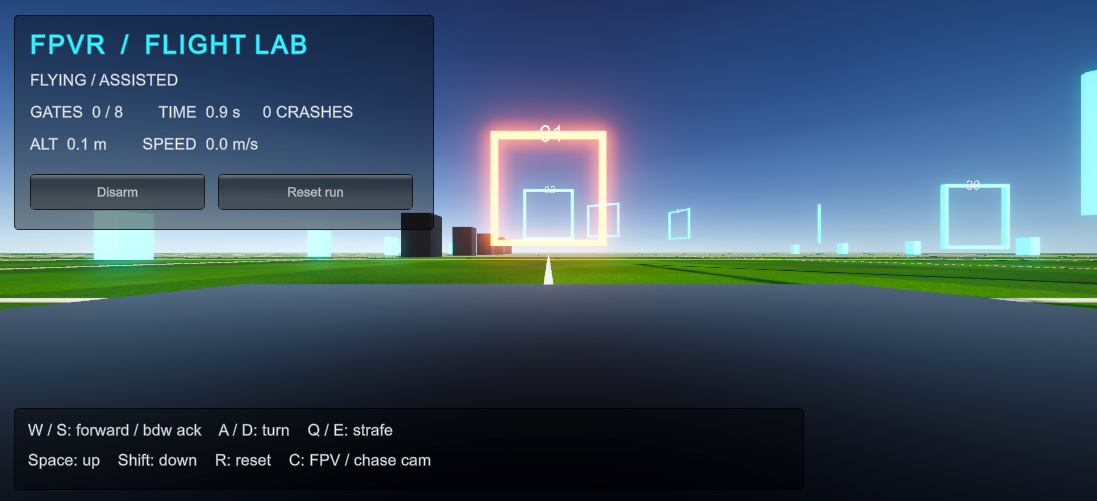
\includegraphics[width=\textwidth]{media/ui_start_course.png}
  \caption{Start Screen for a Demo Course}
\end{figure}
\begin{figure}[H]
  \centering
  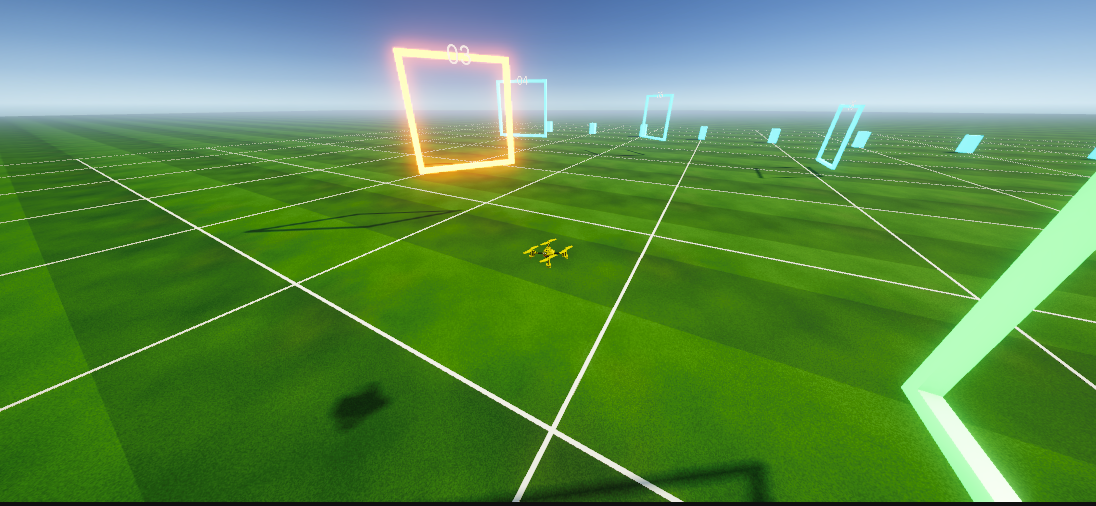
\includegraphics[width=\textwidth]{media/ui_in_flight.png}
  \caption{Drone Flying through Course, 3rd Person View}
\end{figure}
\begin{figure}[H]
  \centering
  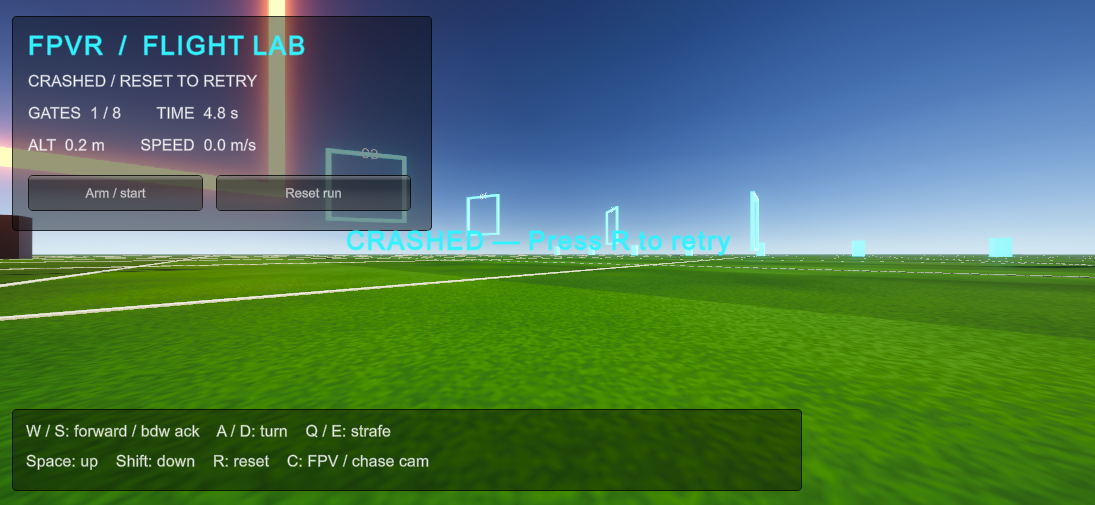
\includegraphics[width=\textwidth]{media/ui_crash_screen.png}
  \caption{Crash Screen}
\end{figure}
\begin{figure}[H]
  \centering
  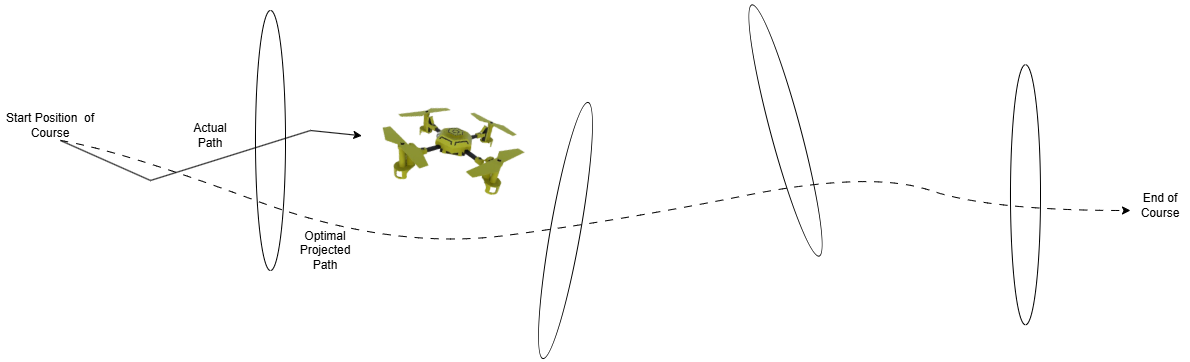
\includegraphics[width=\textwidth]{media/ui_path_diagram.png}
  \caption{Crude Diagram of Optimal Path Generation for a Course}
\end{figure}

\subsection{Hardware User Interfaces}
\begin{figure}[H]
  \centering
  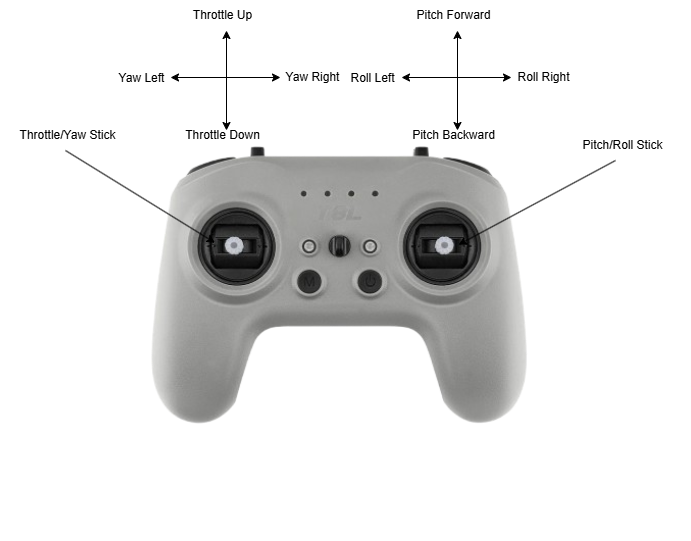
\includegraphics[width=\textwidth]{media/ui_rc_mapping.png}
  \caption{FPV-Style Remote Controller Mappings}
\end{figure}

\section{Design of Communication Protocols}

% \wss{If there is communication between hardware and software, it may be necessary 
% to explain the design of the communication protocol.  This section should be filled 
% in with NA if it is not appropriate for a given project.}
As stated in P.5 of the SRS, if the project were to expand beyond its original scope and
its stretch goals implemented, additional consideration would be required to design a hardware stack
suited for bridging RC communication with FPVR. 

Nearly all drones use a LoRa based radio link for reliable,
long range control and telemetry, and many such RF protocols exist to support this. Among them, the most common open source
protocol is called ExpressLRS (ELRS), which is built on top of Semtech's SX127x/SX1280 LoRa transceivers which can operate in
frequency bands of 900MHz to 2.4GHz. Due to its popularity, platform-agnostic nature, and above average performance compared to 
its competitors, ELRS will be used as the protocol of choice.

\subsection{Hardware Component Diagram}
The overall hardware architecture of the system is depicted in Figure \ref{fig:hardware_component_diagram}.
The E22-M series of chips are variants of the SX1262 transceiver which has additional advantages over its SX127x
predecessors. Specifically, we will be using an E22-900M22S module which operates in 900Mhz and thus
will require a 900Mhz RC transmitter on the controller side. This module is connected to a STM32
microcontroller over SPI running custom ELRS firmware to include support for SX1262 and passing the analog
stick commands through UART to the simulated flight controller in the main application. How this data is formatted
and sent through serial is still to be determined.

\begin{figure}[H]
  \centering
  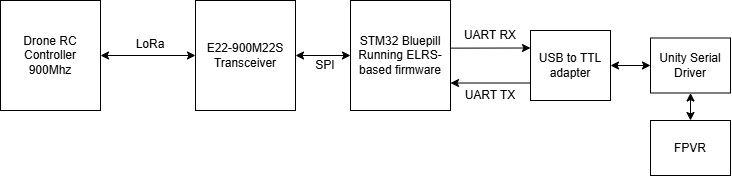
\includegraphics[width=0.8\textwidth]{media/hardware_diagram.png}
  \caption{Hardware Architecture Diagram}
  \label{fig:hardware_component_diagram}
\end{figure}

Unity is capable of communicating with external hardware over serial ports using the \\
\texttt{System.IO.Ports.SerialPort} class provided by the .NET Framework.

\section{Database Design}

\wss{If a database is a significant component of the project, the database
design should be summarized here.  This section should be filled in with NA if
it is not appropriate for a given project.}

\section{Timeline}

\wss{Schedule of tasks and who is responsible}

\wss{You can point to GitHub if this information is included there}

\section{Generative AI Use Disclosure}

Generative AI assisted the review and revision of this Module Guide (MG).
The project team supplied the MG, Software Requirements Specification
(SRS), and MG checklist, then directed revisions through follow-up
instructions. AI produced analysis, replacement text, diagram source, and
supporting SQL drafts. It was not used as evidence that the software meets
its requirements. The following distinguishes work on this revision from
additional drafts prepared during the same editing session.

\subsection{AI Tools Used}

GPT-6.1 and Claude Opus 5.5

\subsection{How and Where Used}

\begin{itemize}
\item \textbf{Requirements and checklist review:} AI compared SRS
functional and quality requirement identifiers with the MG matrix,
explained how requirements inform module responsibilities, and identified
missing or incomplete checklist items. The review addressed anticipated
changes, module secrets, change ownership, dependencies, communication,
and unfinished template sections.
\item \textbf{Architecture revisions:} AI drafted tighter anticipated-change
wording, single-secret module descriptions with grouping justifications,
and corresponding hierarchy, rationale, and traceability updates. It also
proposed separating scoring and leaderboard ordering into additional
modules. These changes affected the sections from Anticipated and Unlikely
Changes through Traceability Matrix in the revised drafts.
\item \textbf{Uses hierarchy:} AI generated helped generate ideas for the hierarchy and provided input and feedback on created designs.
\item \textbf{Communication, database, and schedule drafts:} AI consulted
Unity, Meta, and MySQL documentation, drafted Quest hardware--software
communication text, and revised it to standalone execution following the
team's direction. It drafted a three-relation MySQL design, SQL schema,
query examples, and a relationship diagram. It proposed two activities
per module and start--finish dates, then moved completion to February 15,
2027 at the team's request. These drafts concern Design of Communication
Protocols, Database Design, and Timeline; they are not all incorporated
in this checkout and must not be assumed to describe its present content.
\item \textbf{Editing support:} AI shortened text, aligned terminology and
cross-references, prepared separate local commits, and drafted this
disclosure. The discussion and generated files were review aids; project
scope and acceptance decisions remained with the team.
\end{itemize}

\subsection{Verification of AI-Generated Content}

\begin{itemize}
\item \textbf{Requirements coverage:} Identifier extraction and range
expansion compared the SRS requirements against the MG matrix. The initial
review found all 73 FR/NFR identifiers represented and all 13 original
modules mapped. Revised drafts were checked for coverage of all 73
identifiers, all 15 proposed modules, unique module labels, and valid
module references. These checks establish traceability coverage, not
implementation correctness or proof that each allocation is sufficient.
\item \textbf{Architecture consistency:} The revised PlantUML draft was
checked for 15 nodes and 16 direct edges. Every edge descended its assigned
layer, establishing that this proposed graph had no cycles; each
non-coordinator caller used at most three providers. Ten anticipated-change
rows were checked for one module per row. These results apply to that
draft, not to the unfilled uses figure in the current checkout.
\item \textbf{Technical assertions:} The communication drafts were compared
with official Unity OpenXR input documentation and Meta Link documentation;
the database draft was checked against the MySQL 8.4 table and constraint
documentation. Hardware-specific behaviour and package configuration still
require on-device verification. The SQL was not executed against MySQL
because a server was unavailable; database execution, service authorization,
and retry behaviour therefore remain unverified.
\item \textbf{Document checks:} Revised drafts were compiled with pdfLaTeX
using the existing bibliography, rerunning to resolve cross-references.
Generated diagrams, the database presentation, and schedule pages were
rendered and visually inspected. Git whitespace checks and diff review
were used to detect formatting defects and unintended edits. Compilation
checks LaTeX structure and references; it does not establish factual accuracy.
\item \textbf{Outstanding review:} The current checkout still contains
unfinished sections and differences from the separately verified drafts.
Before submission, the team must reconcile the accepted revisions, resolve
the standalone/PCVR scope discrepancy against the SRS, review each remaining
technical claim and requirement allocation, and repeat compilation and
visual inspection on the actual submission revision. The proposed schedule
also requires confirmation of team capacity. No user study, hardware test,
or independent team sign-off is claimed by this disclosure.
\end{itemize}

The team is responsible for the accuracy, completeness, consistency, and
appropriateness of the submitted MG, including all AI-assisted material.
AI review supplements the team's requirement checks, design review, and
software verification; it does not replace them.

\newpage{}

\bibliographystyle {plainnat}
\bibliography{../../../refs/References}

\end{document}